% === T04 - Circuitos Combinatorios ===
% David Alejandro Gonzalez Marquez
% fokerman@gmail.com
% https://github.com/fokerman/computingSystemsCourse

\documentclass[aspectratio=169]{beamer}
\usepackage{../packages}

\title{\Huge Álgebra de Boole y\\ Circuitos Combinatorios}
\author{David Alejandro González Márquez}
\institute{}

\date{}

\begin{document}

\begin{frame}[plain]
    \titlepage
    \begin{textblock}{100}(30,80)
    \begin{tcolorbox}[size=small,width=\textwidth,colback={gray!30},title={}]
    \begin{center}
     \scriptsize Clase disponible en: \url{https://github.com/fokerman/computingSystemsCourse}
    \end{center}
    \end{tcolorbox}
    \end{textblock}
%     \begin{textblock}{140}(10,70)
%     \textcolor{rojo}{
%     \textbf{Atención}: La clase será grabada por el anfitrión para su posterior y eventual uso académico dentro de nuestra institución. Su participación en la clase implica brindar su consentimiento para participar en la grabación, aunque pueden mantener su video apagado.}
%     \end{textblock}
\end{frame}

\begin{frame}[fragile]
    \frametitle{Circuitos Combinatorios}
    Usando \textbf{compuertas} podemos construir un circuito equivalente a una \textbf{función booleana}.\\
    \bigskip
    A continuación vamos a construir circuitos para realizar \textbf{tareas} específicas.\\
    \bigskip
    \begin{enumerate}
     \item Circuitos Codificadores y Decodificadores
     \item Circuitos Multiplexores y Demultiplexores
     \item Circuitos Aritméticos
    \end{enumerate}
\end{frame}

\begin{frame}[fragile]
    \frametitle{Circuitos Decodificadores y Codificadores}
    \begin{textblock}{100}(10,15) Decodificador \end{textblock}
    \begin{textblock}{100}(10,23) \includegraphics[scale=0.9]{img/cirMuxDemuxCodeDecode-layer4.pdf} \end{textblock}
    \begin{textblock}{100}(50,15)
    \small Circuito que toma $n$ entradas ($\mathrm{e_0}$ a $\mathrm{e_{n-1}}$) y genera $\mathrm{2^n}$ salidas ($\mathrm{s_0}$ a $\mathrm{s_{2^n-1}}$).\\
    \bigskip
    Coloca un \texttt{1} en la salida codificada por la entrada.\\ El resto de las salidas quedan en \texttt{0}.
    \end{textblock}
    \begin{textblock}{100}(10,50)  \only<2->{ \textcolor{gray}{Ejemplo} - \small Decodificador de 2 entradas } \end{textblock}
    \begin{textblock}{100}(3, 60)  \only<2->{ \includegraphics[scale=0.8]{img/exDecoCode-layer1.pdf} } \end{textblock}
    \begin{textblock}{100}(43,60)  \only<2->{ \includegraphics[scale=0.8]{img/exDecoCode-layer2.pdf} } \end{textblock}
    \begin{textblock}{100}(83,60)  \only<2->{ \includegraphics[scale=0.8]{img/exDecoCode-layer3.pdf} } \end{textblock}
    \begin{textblock}{100}(123,60) \only<2->{ \includegraphics[scale=0.8]{img/exDecoCode-layer4.pdf} } \end{textblock}
\end{frame}

\begin{frame}[fragile]
    \frametitle{Circuitos Decodificadores y Codificadores}
    \begin{textblock}{100}(10,15) Codificador \end{textblock}
    \begin{textblock}{100}(10,23) \includegraphics[scale=0.9]{img/cirMuxDemuxCodeDecode-layer3.pdf} \end{textblock}
    \begin{textblock}{100}(50,15)
    \small Circuito que toma $\mathrm{2^n}$ entradas ($\mathrm{e_0}$ a $\mathrm{e_{2^n-1}}$) y genera $n$ salidas ($\mathrm{s_0}$ a $\mathrm{s_{n-1}}$).\\
    \bigskip
    Expone en las salidas la codificación de la única entrada en \texttt{1}.\\ Este circuito no permite que más de una entrada esté en \texttt{1}. 
    \end{textblock}
    \begin{textblock}{100}(10,50)  \only<2->{ \textcolor{gray}{Ejemplo} - \small Codificador de 4 entradas } \end{textblock}
    \begin{textblock}{100}(4,60)  \only<2->{ \includegraphics[scale=0.8]{img/exDecoCode-layer5.pdf} } \end{textblock}
    \begin{textblock}{100}(44,60)  \only<2->{ \includegraphics[scale=0.8]{img/exDecoCode-layer6.pdf} } \end{textblock}
    \begin{textblock}{100}(84,60)  \only<2->{ \includegraphics[scale=0.8]{img/exDecoCode-layer7.pdf} } \end{textblock}
    \begin{textblock}{100}(124,60) \only<2->{ \includegraphics[scale=0.8]{img/exDecoCode-layer8.pdf} } \end{textblock}
\end{frame}

\begin{frame}[fragile]
    \frametitle{Circuitos Decodificadores y Codificadores}
    \begin{textblock}{100}(10,15) \only<1->{ Decodificador } \end{textblock}
    \begin{textblock}{100}(10,23) \only<1->{ \includegraphics[scale=0.9]{img/cirMuxDemuxCodeDecode-layer4.pdf} } \end{textblock}
    \begin{textblock}{100}(51,15) \only<2->{
    \begin{tabular}{|cc|cccc|}  \hline
    \multicolumn{2}{|c|}{\small entradas} & \multicolumn{4}{c|}{\small salida} \\  \hline
    \small\texttt{E$_1$} & \small\texttt{E$_0$} & \small\texttt{S$_0$} & \small\texttt{S$_1$} & \small\texttt{S$_2$} & \small\texttt{S$_3$} \\ \hline
    \small\texttt{0}     & \small\texttt{0}     & \small\texttt{1}     & \small\texttt{0}     & \small\texttt{0}     & \small\texttt{0}     \\
    \small\texttt{0}     & \small\texttt{1}     & \small\texttt{0}     & \small\texttt{1}     & \small\texttt{0}     & \small\texttt{0}     \\
    \small\texttt{1}     & \small\texttt{0}     & \small\texttt{0}     & \small\texttt{0}     & \small\texttt{1}     & \small\texttt{0}     \\
    \small\texttt{1}     & \small\texttt{1}     & \small\texttt{0}     & \small\texttt{0}     & \small\texttt{0}     & \small\texttt{1}     \\ \hline
    \end{tabular} }
    \end{textblock}
    \begin{textblock}{100}(112,15)  \only<3->{ 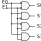
\includegraphics[scale=0.5]{img/decode.pdf} } \end{textblock}
    \begin{textblock}{100}(10,52) \only<1->{ Codificador } \end{textblock}
    \begin{textblock}{100}(10,60) \only<1->{ \includegraphics[scale=0.9]{img/cirMuxDemuxCodeDecode-layer3.pdf} } \end{textblock}
    \begin{textblock}{100}(52,52) \only<4->{
    \begin{tabular}{|cccc|cc|}  \hline
    \multicolumn{4}{|c|}{\small entradas} & \multicolumn{2}{c|}{\small salidas} \\  \hline
    \small\texttt{E$_0$} & \small\texttt{E$_1$} & \small\texttt{E$_2$} & \small\texttt{E$_3$} & \small\texttt{S$_1$} & \small\texttt{S$_0$} \\ \hline
    \small\texttt{1}     & \small\texttt{0}     & \small\texttt{0}     & \small\texttt{0}     & \small\texttt{0}     & \small\texttt{0} \\
    \small\texttt{0}     & \small\texttt{1}     & \small\texttt{0}     & \small\texttt{0}     & \small\texttt{0}     & \small\texttt{1} \\
    \small\texttt{0}     & \small\texttt{0}     & \small\texttt{1}     & \small\texttt{0}     & \small\texttt{1}     & \small\texttt{0} \\
    \small\texttt{0}     & \small\texttt{0}     & \small\texttt{0}     & \small\texttt{1}     & \small\texttt{1}     & \small\texttt{1} \\ \hline
    \end{tabular} }
    \end{textblock}
    \begin{textblock}{100}(112,52)  \only<5->{ 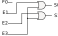
\includegraphics[scale=0.5]{img/encode.pdf} } \end{textblock}
\end{frame}

\begin{frame}[fragile]
    \frametitle{Circuitos Multiplexores y Demultiplexores}
    \begin{textblock}{100}(10,15) Multiplexor \end{textblock}
    \begin{textblock}{100}(10,23) \includegraphics[scale=0.9]{img/cirMuxDemuxCodeDecode-layer1.pdf} \end{textblock}
    \begin{textblock}{100}(50,15)
    \small Circuito que toma $n$ entradas de control ($\mathrm{c_0}$ a $\mathrm{c_{n-1}}$), $\mathrm{2^n}$ entradas de datos ($\mathrm{e_0}$ a $\mathrm{e_{2^n-1}}$) y genera una salida $s_0$.\\
    \bigskip
    Dependiendo del valor de las entradas de control, selecciona una de las entradas de datos y la expone en la salida.
    \end{textblock}
    \begin{textblock}{100}(10,50)  \only<2->{ \textcolor{gray}{Ejemplo} - \small Multiplexor de 4 entradas } \end{textblock}
    \begin{textblock}{100}(10,60)  \only<2->{ \includegraphics[scale=0.8]{img/exMuxDemux-layer1.pdf} } \end{textblock}
    \begin{textblock}{100}(45,60)  \only<2->{ \includegraphics[scale=0.8]{img/exMuxDemux-layer2.pdf} } \end{textblock}
    \begin{textblock}{100}(80,60)  \only<2->{ \includegraphics[scale=0.8]{img/exMuxDemux-layer3.pdf} } \end{textblock}
    \begin{textblock}{100}(115,60) \only<2->{ \includegraphics[scale=0.8]{img/exMuxDemux-layer4.pdf} } \end{textblock}
\end{frame}

\begin{frame}[fragile]
    \frametitle{Circuitos Multiplexores y Demultiplexores}
    \begin{textblock}{100}(10,15) Demultiplexor \end{textblock}
    \begin{textblock}{100}(10,23) \includegraphics[scale=0.9]{img/cirMuxDemuxCodeDecode-layer2.pdf} \end{textblock}
    \begin{textblock}{100}(50,15)
    \small Circuito que toma $n$ entradas de control ($\mathrm{c_0}$ a $\mathrm{c_{n-1}}$), una entrada de datos $\mathrm{e_0}$ y genera $\mathrm{2^n}$ salidas ($\mathrm{s_0}$ a $\mathrm{s_{2^n-1}}$).\\
    \bigskip
    Expone la entrada en una de las salidas, dependiendo del valor de las entradas de control.
    \end{textblock}
    \begin{textblock}{100}(10,50)  \only<2->{ \textcolor{gray}{Ejemplo} - \small Demultiplexor de 4 entradas } \end{textblock}
    \begin{textblock}{100}(10,60)  \only<2->{ \includegraphics[scale=0.8]{img/exMuxDemux-layer5.pdf} } \end{textblock}
    \begin{textblock}{100}(45,60)  \only<2->{ \includegraphics[scale=0.8]{img/exMuxDemux-layer6.pdf} } \end{textblock}
    \begin{textblock}{100}(80,60)  \only<2->{ \includegraphics[scale=0.8]{img/exMuxDemux-layer7.pdf} } \end{textblock}
    \begin{textblock}{100}(115,60) \only<2->{ \includegraphics[scale=0.8]{img/exMuxDemux-layer8.pdf} } \end{textblock}
\end{frame}

\begin{frame}[fragile]
    \frametitle{Circuitos Multiplexores y Demultiplexores}
    \begin{textblock}{100}(10,15) \only<1->{ Multiplexor } \end{textblock}
    \begin{textblock}{100}(10,23) \only<1->{ \includegraphics[scale=0.9]{img/cirMuxDemuxCodeDecode-layer1.pdf} } \end{textblock}
    \begin{textblock}{100}(45,15) \only<2->{
    \begin{tabular}{|cccccc|c|}  \hline
    \multicolumn{6}{|c|}{\small entradas} & \multicolumn{1}{c|}{\small salida} \\  \hline
    \small\texttt{E$_0$} & \small\texttt{E$_1$} & \small\texttt{E$_2$} & \multicolumn{1}{c|}{\small\texttt{E$_3$}} & \small\texttt{C$_1$} & \small\texttt{C$_0$} & \small\texttt{S$_0$} \\ \hline
    \small\texttt{e$_0$} & \small\texttt{e$_1$} & \small\texttt{e$_2$} & \small\texttt{e$_3$} & \small\texttt{0}     & \small\texttt{0}     & \small\texttt{e$_0$} \\
    \small\texttt{e$_0$} & \small\texttt{e$_1$} & \small\texttt{e$_2$} & \small\texttt{e$_3$} & \small\texttt{0}     & \small\texttt{1}     & \small\texttt{e$_1$} \\
    \small\texttt{e$_0$} & \small\texttt{e$_1$} & \small\texttt{e$_2$} & \small\texttt{e$_3$} & \small\texttt{1}     & \small\texttt{0}     & \small\texttt{e$_2$} \\
    \small\texttt{e$_0$} & \small\texttt{e$_1$} & \small\texttt{e$_2$} & \small\texttt{e$_3$} & \small\texttt{1}     & \small\texttt{1}     & \small\texttt{e$_3$} \\ \hline
    \end{tabular} }
    \end{textblock}
    \begin{textblock}{100}(112,15)  \only<6->{ \includegraphics[scale=0.5]{img/muxDemux-layer3.pdf} } \end{textblock}
    \begin{textblock}{100}(112,15)  \only<3->{ \includegraphics[scale=0.5]{img/muxDemux-layer1.pdf} } \end{textblock}
    \begin{textblock}{100}(10,52) \only<1->{ Demultiplexor } \end{textblock}
    \begin{textblock}{100}(10,60) \only<1->{ \includegraphics[scale=0.9]{img/cirMuxDemuxCodeDecode-layer2.pdf} } \end{textblock}
    \begin{textblock}{100}(47,52) \only<4->{
    \begin{tabular}{|ccc|cccc|}  \hline
    \multicolumn{3}{|c|}{\small entradas} & \multicolumn{4}{c|}{\small salidas} \\  \hline
    \multicolumn{1}{|c|}{\small\texttt{E$_0$}}  & \small\texttt{C$_1$} & \small\texttt{C$_0$} & \small\texttt{S$_0$} & \small\texttt{S$_1$} & \small\texttt{S$_2$} & \small\texttt{S$_3$} \\ \hline
    \small\texttt{e$_0$} & \small\texttt{0}     & \small\texttt{0}     & \small\texttt{e$_0$} & \small\texttt{0}     & \small\texttt{0}     & \small\texttt{0}     \\
    \small\texttt{e$_0$} & \small\texttt{0}     & \small\texttt{1}     & \small\texttt{0}     & \small\texttt{e$_0$} & \small\texttt{0}     & \small\texttt{0}     \\
    \small\texttt{e$_0$} & \small\texttt{1}     & \small\texttt{0}     & \small\texttt{0}     & \small\texttt{0}     & \small\texttt{e$_0$} & \small\texttt{0}     \\
    \small\texttt{e$_0$} & \small\texttt{1}     & \small\texttt{1}     & \small\texttt{0}     & \small\texttt{0}     & \small\texttt{0}     & \small\texttt{e$_0$} \\ \hline
    \end{tabular} }
    \end{textblock}
    \begin{textblock}{100}(112,52)  \only<6->{ \includegraphics[scale=0.5]{img/muxDemux-layer3.pdf} } \end{textblock}
    \begin{textblock}{100}(112,52)  \only<5->{ \includegraphics[scale=0.5]{img/muxDemux-layer2.pdf} } \end{textblock}
\end{frame}

\begin{frame}[fragile,t]
    \frametitle{Circuitos Aritméticos}
    Conjunto de circuitos que nos permiten realizar \textbf{operaciones matemáticas}.
    \begin{textblock}{60}(8,22)  \only<2->{ \textcolor{naranjauca}{Sumador Simple} } \end{textblock}
    \begin{textblock}{60}(14,27) \only<3->{ \includegraphics[scale=0.8]{img/sumadorOperacion-layer1.pdf} } \end{textblock}
    \begin{textblock}{60}(40,27) \only<4->{ \includegraphics[scale=0.9]{img/sumadorCircuito-layer1.pdf} } \end{textblock}
    \begin{textblock}{100}(64,28)
    \only<5->{
    \renewcommand{\arraystretch}{0.8}
    \begin{tabular}{|C{0.5cm}|C{0.5cm}||C{0.5cm}|C{0.5cm}|}
    \hline
    \small
    $A$ & $B$ & $C_{\texttt{out}}$ & $S$ \\
    \hline
    $0$ & $0$ & $0$ & $0$ \\
    $0$ & $1$ & $0$ & $1$ \\
    $1$ & $0$ & $0$ & $1$ \\
    $1$ & $1$ & $1$ & $0$ \\
    \hline
    \end{tabular}
    }
    \end{textblock}
    \begin{textblock}{100}(112,24)
    \only<6->{
    \small
    $C_{\texttt{out}}$ $=$ $A \cdot B$ \\
    $S$ $=$ $( \overline{A} \cdot B ) + ( A \cdot \overline{B} )$ $=$ $A \oplus B$\\
    }
    \end{textblock}
    \begin{textblock}{60}(112,35) \only<7->{ 
\includegraphics[scale=0.8]{img/sumadorSimple.pdf} } \end{textblock}
    \begin{textblock}{60}(14,60) \only<7->{ \includegraphics[scale=0.8]{img/sumadorOperacion-layer3.pdf} } \end{textblock}
    \begin{textblock}{140}(50,60)
    \only<4->{ Sumador simple de 1 bit, nos permite sumar dos bits \texttt{A} y \texttt{B}.\\
    El resultado se expresa como \texttt{S} y el carry como \texttt{C$_{\texttt{out}}$}.\\ }
    \bigskip
    \only<7->{ \textcolor{verdeuca}{Si queremos sumar más de un bit, necesitamos\\ también sumar el carry de la operación anterior.} }
    \end{textblock}
\end{frame}

\begin{frame}[fragile,t]
    \frametitle{Circuitos Aritméticos}
    \begin{textblock}{60}(8,12) \textcolor{naranjauca}{Sumador Completo} \end{textblock}
    \begin{textblock}{60}(14,20) \only<1->{ \includegraphics[scale=0.8]{img/sumadorOperacion-layer2.pdf} } \end{textblock}
    \begin{textblock}{60}(120,15) \only<2->{ \includegraphics[scale=0.9]{img/sumadorCircuito-layer2.pdf} } \end{textblock}
    \begin{textblock}{65}(43,20)
    \only<2->{Un sumador completo de 1 bit, nos permite sumar dos bits \texttt{A} y \texttt{B}, y además el carry de la operación anterior \texttt{C$_{\texttt{in}}$}.
    El resultado se expresa como \texttt{S} y un carry \texttt{C$_{\texttt{out}}$}.\\ }
    \end{textblock}
    \begin{textblock}{100}(15,47)
    \only<3->{
    \renewcommand{\arraystretch}{0.8}
    \begin{tabular}{|C{0.5cm}|C{0.5cm}|C{0.5cm}||C{0.5cm}|C{0.5cm}|}
    \hline
    $C_{\texttt{in}}$ & $A$ & $B$ & $C_{\texttt{out}}$ & $S$ \\
    \hline
    \small $0$ & \small $0$ & \small $0$ & \small $0$ & \small $0$ \\
    \small $0$ & \small $0$ & \small $1$ & \small $0$ & \small $1$ \\
    \small $0$ & \small $1$ & \small $0$ & \small $0$ & \small $1$ \\
    \small $0$ & \small $1$ & \small $1$ & \small $1$ & \small $0$ \\
    \small $1$ & \small $0$ & \small $0$ & \small $0$ & \small $1$ \\
    \small $1$ & \small $0$ & \small $1$ & \small $1$ & \small $0$ \\
    \small $1$ & \small $1$ & \small $0$ & \small $1$ & \small $0$ \\
    \small $1$ & \small $1$ & \small $1$ & \small $1$ & \small $1$ \\
    \hline
    \end{tabular}
    }
    \end{textblock}
    \begin{textblock}{60}(80,53) \only<3->{ 
\includegraphics[scale=0.8]{img/sumadorCompleto.pdf} } \end{textblock}
\end{frame}

\begin{frame}[fragile,t]
    \frametitle{Circuitos Aritméticos}
    \begin{textblock}{65}(10,13) \only<1->{\textcolor{naranjauca}{Sumador de 4 bits}\\
    Utilizando 4 sumadores completos, podemos construir un sumador de 4 bits.} \end{textblock}
    \begin{textblock}{60}(80,7)  \only<1->{ 
\includegraphics[scale=0.7]{img/sumador4bits.pdf} } \end{textblock}
    
    \begin{textblock}{65}(10,34) \only<2->{\textcolor{naranjauca}{Inversor aditivo de 4 bits}\\
    Si negamos la entrada y le sumamos uno. Obtenemos el inverso aditivo de un número en complemento a 2.} \end{textblock}
    \begin{textblock}{60}(80,31) \only<2->{ 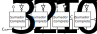
\includegraphics[scale=0.7]{img/inversoAditivo4bits.pdf} } \end{textblock}
    
    \begin{textblock}{65}(10,62) \only<3->{\textcolor{naranjauca}{Restador de 4 bits}\\
    Si sumamos un número con el inverso aditivo de otro obtenemos un circuito restador.} \end{textblock}
    \begin{textblock}{60}(80,60) \only<3->{ 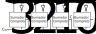
\includegraphics[scale=0.7]{img/restador4bits.pdf} } \end{textblock}
\end{frame}

\begin{frame}[fragile,t]
    \frametitle{Circuitos Aritméticos - Flags}
    \begin{textblock}{57}(5,15)
    \small
    Los circuitos aritméticos además de generar resultados de sus operaciones, también generan lo que se conoce como \textbf{palabra de estado}.\\
    \bigskip
    La palabra de estado contiene\\ una serie de \textbf{Flags}.\\
    \bigskip
    \uncover<2->{Vamos a ver algunos de ellos\\ y cómo se construyen.}
    \end{textblock}
    \begin{textblock}{100}(10,62)
    \begin{tabular}{cc|l}
    \uncover<2->{\textcolor{naranjauca}{N} & Negative & \small Indica si el número es negativo en complemento a 2. \\}
    \uncover<3->{\textcolor{naranjauca}{Z} & Zero & \small Indica si el número es cero en complemento a 2. \\}
    \uncover<4->{\textcolor{naranjauca}{C} & Carry & \small Indica si la operación en complemento a 2 genera acarreo. \\}
    \uncover<5->{\textcolor{naranjauca}{V} & Overflow & \small Indica si el resultado no es representable en complemento a 2. \\}
    \end{tabular}
    \end{textblock}
    \begin{textblock}{60}(65,10) \only<1->{ \includegraphics[scale=0.7]{img/sumador4bitsFlags-layer1.pdf} } \end{textblock}
    \begin{textblock}{60}(65,10) \only<2->{ \includegraphics[scale=0.7]{img/sumador4bitsFlags-layer2.pdf} } \end{textblock}
    \begin{textblock}{60}(65,10) \only<3->{ \includegraphics[scale=0.7]{img/sumador4bitsFlags-layer3.pdf} } \end{textblock}
    \begin{textblock}{60}(65,10) \only<4->{ \includegraphics[scale=0.7]{img/sumador4bitsFlags-layer4.pdf} } \end{textblock}
    \begin{textblock}{60}(65,10) \only<5->{ \includegraphics[scale=0.7]{img/sumador4bitsFlags-layer5.pdf} } \end{textblock}
    \begin{textblock}{60}(65,10) \only<6->{ \includegraphics[scale=0.7]{img/sumador4bitsFlags-layer6.pdf} } \end{textblock}
\end{frame}

\begin{frame}[fragile,t]
    \frametitle{Circuitos Aritméticos - ALU}
    La \textbf{ALU} (\textit{Arithmetic logic unit}) es un circuito combinatorio que toma como entrada operandos e indicaciones de operaciones a realizar, y retorna el resultado de la operación junto con sus flags.
    \vspace{0.2cm}
    \pause
    \begin{center}
    
\includegraphics[scale=0.9]{img/aluBloque.pdf}
    \end{center}
    \pause
    \vspace{-0.7cm}
    \textcolor{gray}{Ejemplo:}
    \begin{center}
    \begin{tabular}{|c|c|c|c|} \hline
    \rowcolor{gray!30} Operando A & Operando B & Operación & Resultado y Flags \\ \hline
    \texttt{A} & \texttt{B} & $+$ & \texttt{A} $+$ \texttt{B} \\ \hline
    \texttt{A} & \texttt{B} & $and$ & \texttt{A} $and$ \texttt{B} \\ \hline
    \texttt{A} & \texttt{B} & $or$ & \texttt{A} $or$ \texttt{B} \\ \hline
    \texttt{A} & \texttt{}  & $not$ & $\overline{\text{A}}$ \\ \hline
    \end{tabular}
    \end{center}
\end{frame}

\begin{frame}[fragile,t]
    \frametitle{Circuitos Aritméticos - ALU de 1 bit}
    \begin{textblock}{60}(15,17) \only<7-17>{  \includegraphics[scale=0.6]{img/alu1bitCompleta-layer7.pdf}  } \end{textblock} % Bloques
    \begin{textblock}{60}(15,17) \only<8-17>{  \includegraphics[scale=0.6]{img/alu1bitCompleta-layer8.pdf}  } \end{textblock} % wire A
    \begin{textblock}{60}(15,17) \only<9-17>{  \includegraphics[scale=0.6]{img/alu1bitCompleta-layer9.pdf}  } \end{textblock} % wire B
    \begin{textblock}{60}(15,17) \only<10-17>{ \includegraphics[scale=0.6]{img/alu1bitCompleta-layer10.pdf} } \end{textblock} % resultados
    \begin{textblock}{60}(15,17) \only<11-17>{ \includegraphics[scale=0.6]{img/alu1bitCompleta-layer11.pdf} } \end{textblock} % Select
    \begin{textblock}{60}(15,17) \only<12-17>{ \includegraphics[scale=0.6]{img/alu1bitCompleta-layer12.pdf} } \end{textblock} % Decode
    \begin{textblock}{60}(15,17) \only<13-17>{ \includegraphics[scale=0.6]{img/alu1bitCompleta-layer13.pdf} } \end{textblock} % NOT
    \begin{textblock}{60}(15,17) \only<14-17>{ \includegraphics[scale=0.6]{img/alu1bitCompleta-layer14.pdf} } \end{textblock} % OR
    \begin{textblock}{60}(15,17) \only<15-17>{ \includegraphics[scale=0.6]{img/alu1bitCompleta-layer15.pdf} } \end{textblock} % AND
    \begin{textblock}{60}(15,17) \only<16-17>{ \includegraphics[scale=0.6]{img/alu1bitCompleta-layer16.pdf} } \end{textblock} % SUM
    \begin{textblock}{60}(15,17) \only<17->{   \includegraphics[scale=0.6]{img/alu1bitCompleta-layer17.pdf} } \end{textblock} % Zero
    \begin{textblock}{60}(15,17) \only<18->{   \includegraphics[scale=0.6]{img/alu1bitCompleta-layer18.pdf} } \end{textblock} % COLOR
    \begin{textblock}{60}(15,17) \only<2->{    \includegraphics[scale=0.6]{img/alu1bitCompleta-layer2.pdf}  } \end{textblock} % Operandos A B
    \begin{textblock}{60}(15,17) \only<3->{    \includegraphics[scale=0.6]{img/alu1bitCompleta-layer3.pdf}  } \end{textblock} % Resultado S
    \begin{textblock}{60}(15,17) \only<4->{    \includegraphics[scale=0.6]{img/alu1bitCompleta-layer4.pdf}  } \end{textblock} % Operacion
    \begin{textblock}{60}(15,17) \only<5->{    \includegraphics[scale=0.6]{img/alu1bitCompleta-layer5.pdf}  } \end{textblock} % Operacion A B tabla
    \begin{textblock}{60}(15,17) \only<6->{    \includegraphics[scale=0.6]{img/alu1bitCompleta-layer6.pdf}  } \end{textblock} % Flags / carry
    \begin{textblock}{60}(15,17) \only<1->{    \includegraphics[scale=0.6]{img/alu1bitCompleta-layer1.pdf}  } \end{textblock} % Borde
\end{frame}

\begin{frame}[fragile,t]
    \frametitle{Lógica de tres estados}
    \begin{textblock}{60}(10,15)
    \small 
    \only<1->{ Supongamos tener un \textbf{cable} que conecta tres circuitos diferentes. Si un circuito escribe una señal, esta es leída por los otros.\\ }
    \bigskip
    \only<2->{ Ahora, no es posible que dos circuitos escriban \textbf{simultáneamente} una señal.\\ }
    \bigskip
    \only<3->{ A pesar de que los circuitos puedan acordar no escribir simultáneamente.\\
    \bigskip Necesitaríamos algún dispositivo que \textbf{permita decidir} si leemos o escribimos un cable.\\ }
    \end{textblock}
    \begin{textblock}{60}(80,15) \only<1->{ \includegraphics[scale=0.9]{img/busExample-layer1.pdf} } \end{textblock}
    \begin{textblock}{60}(80,35) \only<2->{ \includegraphics[scale=0.9]{img/busExample-layer2.pdf} } \end{textblock}
    \begin{textblock}{60}(80,55) \only<3->{ \includegraphics[scale=0.9]{img/busExample-layer3.pdf} } \end{textblock}
    \begin{textblock}{140}(10,78)
    \only<4->{ \textcolor{verdeuca}{No podemos cambiar el cable para leer o escribir, pero sí podemos \textbf{desconectarlo}.} } 
    \end{textblock}
\end{frame}

\begin{frame}[fragile,t]
    \frametitle{Lógica de tres estados}
    \begin{textblock}{80}(10,15)
    \small 
    \only<1->{ Un componente de 3 estados es un circuito electrónico que presenta a su salida tres estados posibles:\\
    \begin{itemize}
    \setlength\itemsep{0cm}
     \item[\textcolor{naranjauca}{\texttt{0}}] Estado lógico Cero.
     \item[\textcolor{naranjauca}{\texttt{1}}] Estado lógico Uno.
     \item[\textcolor{naranjauca}{\texttt{hi-Z}}] No estado. Desconectado (\emph{Alta impedancia}).
    \end{itemize} }
    \only<2->{ 
    \begin{center}
    \begin{tabular}{cc|c}
    \texttt{C} & \texttt{E} & \texttt{S} \\ \hline
    \texttt{0} & \texttt{0} & \texttt{hi-Z} \\
    \texttt{0} & \texttt{1} & \texttt{hi-Z} \\ \hline
    \texttt{1} & \texttt{0} & \texttt{0} \\
    \texttt{1} & \texttt{1} & \texttt{1} \\ \hline
    \end{tabular}
    \end{center} }
    \end{textblock}
    \begin{textblock}{60}(100,20) \only<1->{ \includegraphics[scale=1]{img/3state-layer1.pdf} } \end{textblock}
    \begin{textblock}{60}(85,50)  \only<2->{ \includegraphics[scale=0.8]{img/3state-layer3.pdf} } \end{textblock}
    \begin{textblock}{60}(115,50)  \only<2->{ \includegraphics[scale=0.8]{img/3state-layer2.pdf} } \end{textblock}
    \begin{textblock}{140}(10,68)
    \small
    \only<3->{ Este componente nos permite \textbf{desconectar} circuitos, para así decidir cuándo escribir o leer de un cable.\\ }
    \bigskip
    \only<4->{ \textbf{Más adelante:}\\ \textcolor{verdeuca}{ Vamos a construir registros bidireccionales y utilizar buses, donde usaremos este componente.} } 
    \end{textblock}
\end{frame}

\begin{frame}[fragile]
    \frametitle{Bibliografía}
    \begin{itemize}
     \setlength\itemsep{0.5cm}
    \item[-] \small Tanenbaum, “Organización de Computadoras. Un Enfoque Estructurado”, 4ta Edición, 2000.\\
    \begin{itemize}
     \item \textbf{Capítulo 3 - El nivel de lógica digital} - Páginas 128-139
    \end{itemize}
    \item[-] \small Null, “Essentials of Computer Organization and Architecture”, 5th Edition, 2018.\\
    \begin{itemize}
     \item \textbf{Chapter 3 - Boolean Algebra and Digital Logic:}
     \begin{itemize}
     \item 3.6 - Combinational Circuits
     \end{itemize}
    \end{itemize}
%     \item[-] \small Silberschatz, “Fundamentos de Sistemas Operativos”, 7ma Edición, 2006.\\
%     \item[-] \small Tanenbaum, “Modern Operating Systems”, 4th Edition, 2015.\\
    \end{itemize}
\end{frame}

\begin{frame}[fragile]
    \frametitle{Ejercicios}
    Con lo visto, ya pueden resolver hasta el ejercicio 9 de la Guía de Lógica Digital.
\end{frame}

\begin{frame}[plain]
    \begin{center}
    \vspace{2cm}
    \huge ¡Gracias!\\
    \vspace{2cm}
    \normalsize Recuerden leer los comentarios adjuntos\\ en cada clase por aclaraciones.
    \end{center}
\end{frame}

\end{document}

% % % % % % % % % % % % % % % % % % 
% EJEMPLOS:

\begin{frame}[fragile]
    \frametitle{Bla}
    \begin{itemize}
    \item[-] Bla bla \textbf{ble} bla bla
    \item[-] Bla bla \textbf{ble} bla bla
    \end{itemize}
\end{frame}

\begin{frame}[fragile]
    \frametitle{Bla}
    \begin{block}{\texttt{BLA}}
    Bla Bla
    \end{block}
    \begin{multicols}{2}
    \begin{tabular}{ll}
    la & la \\
    \end{tabular}
    \columnbreak
    \begin{tabular}{ll}
    la & la \\
    \end{tabular}
    \end{multicols}
\end{frame}

\begin{frame}
    \frametitle{Bla}
    \begin{itemize}
    \item Bla bla
    \begin{center}
    \includegraphics[scale=0.7]{img/struct_aling.pdf}
    \end{center}
    Bla bla
    \end{itemize}
\end{frame}

\begin{frame}[fragile]
    \frametitle{Bla}
    \begin{textblock}{100}(10,10)
    Bla
    \end{textblock}
\end{frame}

\end{document}

